\cotefile{156-9}
\scanpage{2}
% archive sheet number: 1
% top right
\hfill GF \uline{$\overline{\mathrm{IX}}$}

\margin{(voir p \unsure{75} la mise au pt sur la terminologie\unsure{)}}

\diagram{%
\begin{tikzcd}[ampersand replacement=\&,column sep=small,row sep=large,execute at end picture={\draw[gray,line width=1.2pt] (sepA.center)--(sepB.center);}]
\& \& \begin{gathered}\text{Atelier général}\quad\text{\textcircled{$\unsure{\mathscr A|\mathcal A}$}}\\(\mathscr A,\unsure{\unlhd|\trianglelefteq},\ll,|\circ|)\end{gathered}
 \arrow[dll,dash] \arrow[dl,dash] \arrow[dr,dash] \arrow[drr,dash] \arrow[dddrr,bend left=35] \& \& \\
\begin{gathered}\text{\uline{atelier spatial}}\\(\mathscr A_{\unsure{\varphi}},\unlhd,|\circ|)\quad\text{\textcircled{$\Sigma$}}\end{gathered}
 \arrow[dr,dash] \arrow[ddrr] \arrow[dddrrr,dashed,dash]
 \& \begin{gathered}\text{\deleted{\uline{\unsure{Atlier|Atelier} divisé}}}\\\text{\uline{atelier local}}\\(\mathscr A,\unlhd,\ll,|\circ|_{\unsure{\ll}})\end{gathered}\arrow[d,dash]
 \& \& \begin{gathered}\text{\uline{atelier fidèle}}\\(\mathscr A,\unlhd,\ll)\end{gathered}\arrow[dll,dash]\arrow[ddd]
 \& \text{\deleted{atelier modéré}}\\
\& \begin{gathered}\text{\uline{atelier ponctuel}}\\\Sigma\simeq\unsure{\mathscr P|\mathcal P}(2)\end{gathered}\arrow[dr]\arrow[rr,dashed,dash,bend right=30,"?"']
 \& \& \text{\uline{at. mod}\ ?} \& \\
\& \& \begin{gathered}\text{\textcircled{$\unsure{\mathscr L|\mathcal L}$}}\ \text{\uline{atelier ensembliste}}\end{gathered}\arrow[d]
 \& \& \text{atelier modéré}\arrow[dl]\arrow[dll,dashed]\\
\& \& \text{\uline{at. ens. modéré}}\arrow[dd]
 \& \begin{gathered}\text{maquette}\ \Sigma\simeq\mathscr P(\mathscr A)\end{gathered}\arrow[ddl] \& \\
|[alias=sepA]|{} \& \& \& \& |[alias=sepB]|{} \\
\& \& \text{at. \uline{discret}}\arrow[d]\& \& \\
\& \& \begin{gathered}\text{\deleted{\unsure{at. final}}}\\\text{\uline{at.-point}}\end{gathered}\& \&
\end{tikzcd}}
\margin{\figure{\begin{tikzpicture}
\node[anchor=north west,inner sep=1pt,text width=\marginparwidth,align=left] (note) at (0,0) {\uline{NB} Si les ateliers mod sont fidèles, le diagramme se simplifie \unsure{at mod se place} entre at fid et maq.};
\draw[gray] ([xshift=-2mm,yshift=2mm]note.north west) .. controls ([xshift=8mm,yshift=3mm]note.north west) and ([xshift=-6mm,yshift=3mm]note.north east) .. ([xshift=2mm,yshift=0mm]note.north east) -- ([xshift=2mm,yshift=-2mm]note.south east) .. controls ([xshift=-6mm,yshift=-2mm]note.south east) and ([xshift=6mm,yshift=-2mm]note.south west) .. ([xshift=-2mm,yshift=-2mm]note.south west);
\end{tikzpicture}}}

Je \unsure{me suis intéressé} plus particulièrement \inserted{\unsure{donc}} \unsure{par|pour} les ateliers \uline{spatiaux} \inserted{(Si on \unsure{veut}!)}, incluant les ateliers ensemblistes, comme ceux définis par des \deleted{\unsure{ens. ord.}} ``ensembles ordonnés'', et les maquettes. (at. sp. \unsure{locaux}).

Parmi ceux-ci, pour un travail \inserted{\unsure{primaire} par certains côtés,} proche de l'\unsure{impact} de la topologie ensembliste, je suis intéressé par les ateliers qui sont de plus locaux. (Cela exclut les maquettes, parmi les exemples précédents, sauf les maquettes discrètes).

En développant \unsure{d'abord} une topologie modérée, je m'intéresserai aux \uline{ateliers modérés} (\unsure{ensemblistes} ou non) -- qui incluent les maquettes. Je présume qu'il y a lieu \deleted{\unsure{de s'imposer}} pour les ateliers modérés \deleted{\unsure{qu'ils soient}} \inserted{d'être \uline{\unsure{spatiaux}} (\unsure{voire} pas néc. locaux)}, et peut être
% stamp: TSUP

\scanpage{3}
% archive sheet number: 2
% left half, continuation
\unsure{aussi} que l'ensemble \inserted{ordonné} $\Sigma$ des supports soit ``modulaire'' i.e. $A\wedge\operatorname{Sup}_{i} B_i=\operatorname{Sup}_{i} A\wedge B_i$, donc une ``algèbre de Boole''. Il est possible que cela implique que l'atelier est aussi fidèle.
% slanted
\margin{\figure{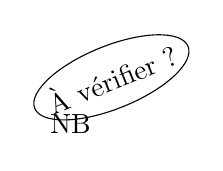
\begin{tikzpicture}
\node[rotate=22,align=center] at (0,0) {\unsure{À vérifier}\ ?};
\draw[rotate=22] (0,0) ellipse (1.05cm and .4cm);
\node[anchor=north west] at (-.9,-.35) {\deleted{\unsure{NB}}};
\end{tikzpicture}}}

\uline{Question} Si $x\in\unsure{\mathscr L|\mathcal L}$, alors $x^\circ=\unsure{\operatorname{supp}^\circ|\operatorname{sup}^\circ} x=\operatorname{supp}\unsure{x}\in\Sigma$ est-il un objet minimal de $\Sigma^{\unsure{*}}=\Sigma\setminus\{0_\Sigma\}$ ? En d'autres termes, si $X\in\unsure{\mathscr A|\mathcal A}$, $\deleted{\unsure{X\notin\mathscr L}}$, et si $\operatorname{supp}^\circ X\subset\operatorname{supp}^\circ x$, a-t-on $X=x$. En d'autres termes
\[
X\ne x\overset{?}{\Longrightarrow}\operatorname{supp}^\circ(\unsure{x|X})\unsure{\not\subset}\operatorname{supp}^\circ x
\quad\text{\uuline{i.e.}}\quad
\operatorname{cosupp}^\circ x\unsure{\not\subset}\operatorname{cosupp}^\circ X
\]
i.e. $\exists Z\in\mathscr A$ avec $Z|\circ|x$, $Z\overline{|\circ|}X$ ? Si c'est un local, on se ramène au cas $X=y\in\mathscr L$, (car
\[
X^\circ=\underset{\substack{y\in\mathscr L,\\\text{t.q. }y\unsure{\ll}X\\\text{i.e. }y^\circ\subset X^\circ}}{\operatorname{Sup}}y
\]
), donc à voir si $x,y\in\mathscr L$, $y\ne x$, $\exists Z\in\mathscr A$ avec $Z|\circ|x$, $Z\overline{|\circ|}y$. Je n'y \unsure{ai pensé|arrive} que dans le cas $x\overline{|\circ|}y$.

\margin{\uline{15.7.}}
\uline{Requestion :} Opération de saturation d'un atelier, \unsure{en sens contraire}, faisable dans le cadre des ateliers spatiaux sans plus ? J'en doute !

\diagram{\begin{tikzcd}[ampersand replacement=\&,row sep=small,column sep=small]
\& |[circle,draw,inner sep=1pt]|{S}\arrow[ddl,dash,bend right=30,line width=1.4pt]\arrow[dr,dash]\arrow[ddd,dash]\&\\
\deleted{\unsure{M}}\&\&|[circle,draw,inner sep=1pt]|{LS}\arrow[ddd,dash,line width=1.2pt]\\
|[circle,draw,inner sep=1pt]|{M}\arrow[dddr,dash,bend right=20,line width=1.2pt]\arrow[uur,dash,gray]\&\&\\
\&SF\arrow[dd,dash]\arrow[dr,dash,line width=1.2pt]\&\\
\&\& E\arrow[dd,dash,line width=1pt]\\
\&\unsure{MF}\arrow[dd,dash,line width=1pt]\arrow[dr,dash,line width=1pt]\&\\
\&\&|[circle,draw,inner sep=1pt]|{EM}\\
\&Mq\&
\end{tikzcd}}
\margin{$D\ E\ G\ \unsure{C|E}\ F\ L\ M\ P\ S$\\$Mq,Di,\unsure{v|\nu},p$}

% right half, reused handwritten cover
\hfill\uline{n° 574}

\hfill\uline{300 exemplaires}

Fascicule 0

Recto verso

1) Page de garde

2) Lettre\qquad L 1 à L 43

3) Table des Matières\qquad T 1 : T 10

Les trois dernières pages de la table des matières sont tirées avec le fascicule 4

(à \unsure{600|500} exemplaires)

4) Introduction\qquad (i à cxxii)

\hfill M\textsuperscript{me} LACAN

% slanted lower-left note on the right half
\figure{\begin{tikzpicture}[rotate=28]
\draw (0,0)--(2,0) (0,-.13)--(0,.13) (2,-.13)--(2,.13);
\draw (2,.12)--(4,.12) (2,0)--(2,.25) (4,0)--(4,.25);
\node at (1,-.3){$S$};\node at (3,.43){$T$};
\draw (-.5,-.4)--(-.5,-.7)--(4.4,-.7)--(4.4,-.4);
\end{tikzpicture}}
\margin{$S\wedge T=S\wedge\underbrace{\underbrace{C(1\wedge C^T)}_{C^T}}_{T}=$\\$\deleted{\unsure{A}}$\\$1-C^T$}

\scanpage{4}
% archive sheet number: 3
% Left half blank apart from the archive number.
Diagramme des principaux types d'ateliers (ou de ``contrées'').

15 juillet 86

\diagram{\begin{tikzcd}[ampersand replacement=\&,column sep=small,row sep=small,
execute at end picture={\begin{scope}\clip (s.center)--(ls.center)--(em.center)--(m.center)--cycle;\foreach \n in {-25,...,25}{\draw[gray,opacity=.45] (\n,-20)--++(20,30);}\end{scope}}]
\&\&\bullet\ G\ (\unsure{\mathscr A|\mathcal A})\&\&\\
\&\&\&\bullet\ \unsure{Div}\arrow[ul]\&\\
|[alias=s,circle,draw]|{S\ \bullet}\ (\Sigma\text{ ou }\mathscr A)\arrow[uurr]\&\&\&\&\bullet\ L\arrow[ul]\\
\&\&\bullet\ F\arrow[uuu,line width=1.2pt]\&\&\\
\&\&|[alias=ls,circle,draw,double]|{LS\ \bullet}\ (\Sigma\text{ ou }\unsure{\mathscr L|\mathcal L})\arrow[uull,line width=1.4pt,"{[SDiv]}"{name=sdiv,description}]\arrow[uurr,line width=1.4pt]\&\&\\
SF\ \bullet\arrow[uuu,line width=1.2pt]\arrow[uurr,line width=1.4pt]\&\&\&\&\bullet\ FL=P\arrow[uuu,line width=1.2pt]\arrow[uull,dashed]\\
\&\&\text{\textcircled{$\bullet$}}\ FLS=E\ (\mathscr L)\arrow[uu]\arrow[ull,line width=1.2pt]\arrow[urr,line width=1.4pt]\&\&\\
|[alias=m,circle,draw,double]|{M\ \bullet}\arrow[uu,line width=1.2pt]\&\&\deleted{\unsure{E}}\&\&\\
\&\&|[alias=em,circle,draw]|{\bullet\ EM}\arrow[uu,line width=1.6pt]\arrow[ull,line width=1.5pt]\&\&\\
Mq\ \bullet\arrow[uu,line width=1.4pt]\&\&\&\&\\
\&\&\bullet\ D\arrow[ull,line width=1.3pt]\arrow[uu,line width=1.3pt]\&\&\\
\&\&\&\unsure{\mathscr S}\&\\
\&v\arrow[uur,bend left=15,line width=1.2pt]\&p\arrow[uu,line width=1.2pt]\&\&
\arrow[from=2-4,to=sdiv,dotted,dash]
\end{tikzcd}}
\margin{À vérifier que la bonne notion d'\uline{atelier modéré} doit bien impliquer qu'il est, non seulement \uline{spatial} mais encore, \uline{fidèle}. Sinon, diagramme moins joli ! (Cf ci-contre, feuille \unsure{voisine}.)}

\uline{Légende :}
\[
\begin{array}{rcll}
G&=&\text{ateliers généraux}\\
S&=&\text{--- spatiaux}\\
F&=&\text{--- fidèles}\\
L&=&\text{--- locaux}\\
SF&=&\text{--- spatiaux locaux}\\
FL=P&=&\text{--- fidèles locaux}\\
&&\text{ou \uline{ponctuaires}}\\
LS&=&\text{--- locaux spatiaux}\\
&&\text{\inserted{$\overset{?}{\longrightarrow}$ (NB $LS=S\cap Div$, at. spatiaux divisibles).}}\\
FLS=E&=&\text{--- fidèles locaux spatiaux}\\
&&\text{ou \uline{ensemblistes}}\\
M&=&\text{--- modérés}\\
EM&=&\text{--- ensemblistes \inserted{(modérés)}}\\
Mq&=&\text{--- -maquettes}\\
D&=&\text{--- discrets}\\
Div&=&\text{--- (infiniment) \uline{divisibles}}\\
SDiv&=&\text{--- spatiaux (inf.)}\\
p&\equiv&\text{\deleted{atelier} ponctuels}\quad(\operatorname{card}A=1)\\
v&=&\text{--- vide}\ (\operatorname{card}A=0).
\end{array}
\]

\diagram{\begin{tikzcd}[ampersand replacement=\&,row sep=small,column sep=small]
\&d\&\\b\arrow[ur]\&\&c\arrow[ul]\\\&a\arrow[ul]\arrow[ur]\&
\end{tikzcd}}
Les huit ``carrés élémentaires'' figurant dans ce diagramme sont des ``carrés-intersection'', i.e. $a=b\cap c$. On en conclut p.ex., par ``chasse'', que $LS\cap M=EM\ (=E\cap M)$.

$\deleted{\unsure{L\cap F\cap M}}$

Les cadres privilégiés par excellence pour une ``géométrie des formes'' dans une ``contrée'' me semblent à présent : $LS$ \inserted{$(\overset{?}{=}S\cap Div)$} (ateliers locaux-spatiaux), \deleted{ou mieux, spatiaux divisibles} \deleted{\unsure{toutefois}} qui semblent adéquats pour l'étude des \deleted{\illegible{2}} \inserted{\unsure{cordes et}} pseudo-\unsure{simplexes} topologiques; $S$ (ateliers spatiaux) \inserted{adéquats \unsure{(a priori)} pour les contrées finies)} $M$ (ateliers modérés, pour la topologie modérée) et $EM$ (topologie modérée ensembliste\unsure{)}

\margin{\figure{\begin{tikzpicture}
\node[anchor=north west,inner sep=1pt,text width=\marginparwidth,align=left] (note) at (0,0) {Je note que l'accent principal s'est nettement déplacé, depuis les approches originelles via $L$, vers des \deleted{\unsure{appro}}\unsure{approches très subordonnées} à $S$ (le dernier venu dans la trilogie $FLS$).};
\draw[gray] ([xshift=-2mm,yshift=2mm]note.north west) .. controls ([xshift=8mm,yshift=3mm]note.north west) and ([xshift=-6mm,yshift=3mm]note.north east) .. ([xshift=2mm,yshift=0mm]note.north east) -- ([xshift=2mm,yshift=-2mm]note.south east) .. controls ([xshift=-6mm,yshift=-2mm]note.south east) and ([xshift=6mm,yshift=-2mm]note.south west) .. ([xshift=-2mm,yshift=-2mm]note.south west);
\end{tikzpicture}}}

\scanpage{5}
\mspage{1}
% archive sheet number: 4
\deleted{\unsure{219|29}}

\uline{5 juillet} L'affaire a tendance à s'enliser, et j'ai envie de tout reprendre, d'une façon \deleted{\unsure{critique}} un peu différente.

\unsure{N} Si $L$ est un ensemble ordonné, je lui associe la maquette \deleted{\unsure{A}}
\[
\unsure{\mathscr M|\mathcal M}=\mathscr M_0\amalg\mathscr M_1
\]
\inserted{$I_{a,b}$}
\[
\begin{aligned}
\mathscr M_0&=L,\quad\text{ensemble des ``\uline{sommets}'' virtuels, ou ``\uline{lieux}''.}\\
\mathscr M_1&\unsure{\overset{\mathrm{d\acute ef}}{=}}\operatorname{Drap}_2(L).
\end{aligned}
\]
Si $\{a,b\}$ $(a<b)$ est un $\operatorname{Drap}_2(L)$, je note $I_{\{a,b\}}$ ou $I_{a,b}$ ou $I_{b,a}$ la strate associée, appelée aussi \uline{intervalle} déterminé par $\{a,b\}$.
% slanted
\margin{On suppose $L$ connexe, $\operatorname{card}L\geq2$.}

\deleted{Relation d'incidence : $X\triangleleft Y$ ssi $X\in$}

Notation $\partial X$, $X\in\mathscr M$ :
\[
\text{\textcircled{a}}\quad
\begin{cases}
\partial I_{\{a,b\}}=\{a,b\}\subset\mathscr M_0\\
\partial x=\varnothing\subset\mathscr M
\end{cases}
\qquad
\text{\textcircled{b}}\quad
\begin{cases}
\delta I_{a,b}=\partial I_{a,b}=\{a,b\}\\
\delta x=\{x\}
\end{cases}
\]
% slanted
\margin{support ``naïf''\par
$c\ \left\{\begin{aligned}|I_{a,b}|^{\unsure{\circ}}&=[a,b]=\{x\in L\mid a\leq x\unsure{\leq b}\}\\|a|&=\{a\}\end{aligned}\right.$\par
$d)\quad |X|^\circ=|X|\setminus\partial X\ \begin{cases}]a,b[&\text{si }X=\unsure{I_{a,b}}\\\{a\}&\text{si }X=a\end{cases}$\par
Notons, pour $X\in\mathscr M$, $\delta X$ et $\partial X\subset L$, mais $\partial X\subset\delta X$.}

\uline{Relation d'incidence :} $X\triangleleft Y$ ssi $X\unsure{\equiv|=}x\in L$, $Y\in\mathscr M_1$, et $x\in\partial Y$. Donc la notion $\partial X$ du début est celle associée à cette relation d'incidence
\[
\partial X=\{Y\in\mathscr M\mid Y\triangleleft X\}\qquad(X\in\mathscr M)
\]
[Il semble qu'il soit mieux introduire d'abord la relation $\leq$ sur $\mathscr M$, d'interpréter $\deleted{\unsure{I_{a,b}}}$, $I_{a,b}^\circ$, $I_{<a}$, $I_{>b}$ comme des ``intervalles'' de $\mathscr M$, i.e. les \unsure{sous-ensembles} via $\unsure{\mathrm{Ord}^\circ}$.]

Relation $\ll$. On a par définition
\[
X\overset{\circ}{\ll}Y\Longleftrightarrow |X|\subset|Y|\quad\text{et}\quad\deleted{\unsure{X\ne Y}}\ X\overline{\triangleleft}Y.
\]
\[
X\overset{\circ}{\ll}Y\Longleftrightarrow
\begin{cases}
X=Y\\
\text{ou }X=x\in L,\ Y=I_{a,b},\quad a<x<b\\
\text{ou }X=I_{a,b},\ Y=I_{a',b'},\quad a'\leq a<b\leq b'
\end{cases}
\]
\margin{\figure{\begin{tikzpicture}
\node[anchor=north west,inner sep=1pt,text width=\marginparwidth,align=left] (note) at (0,0) {Relat\textsuperscript{n} d'ordre\par\uline{Maq $2,\deleted{\unsure{4}}$OK}};
\draw[gray] ([xshift=-2mm,yshift=2mm]note.north west) .. controls ([xshift=8mm,yshift=3mm]note.north west) and ([xshift=-6mm,yshift=3mm]note.north east) .. ([xshift=2mm,yshift=0mm]note.north east) -- ([xshift=2mm,yshift=-2mm]note.south east) .. controls ([xshift=-6mm,yshift=-2mm]note.south east) and ([xshift=6mm,yshift=-2mm]note.south west) .. ([xshift=-2mm,yshift=-2mm]note.south west);
\end{tikzpicture}}}

\figure{\begin{tikzpicture}
\node[anchor=north west,inner sep=0pt] (body) at (0,0) {\begin{minipage}{.86\linewidth}
\uline{Remarque}\quad
$X\overset{\deleted{\unsure{\circ}}}{\ll}Y\Longrightarrow\delta X\cup\delta Y\in\operatorname{Drap}(L)$

\uline{Conséquence}\quad Relation $X\overset{\deleted{\unsure{\circ}}}{\ll}Y$ $(\overset{\mathrm{d\acute ef}}{\Longleftrightarrow}\exists Y',\ X\overset{\circ}{\ll}Y'\unsure{\unlhd|\trianglelefteq} Y)$
\[
\begin{aligned}
X\ll Y&\Longleftrightarrow\deleted{\unsure{X=Y}}\ \text{ou}\ \underbrace{X\triangleleft Y\ \text{ou}\ X\overset{\circ}{\ll}Y}_{\text{\deleted{\unsure{mut}}mutuellement exclusifs}}\Longleftrightarrow|X|\subset|Y|\\
&\Longleftrightarrow\begin{cases}
X=Y\\
\text{ou }X=x\in L,\ Y=I_{a,b},\quad a\leq x\leq b\\
\text{ou }X=I_{a,b},\ Y=I_{a',b'},\quad a'\leq\unsure{a}<b\leq b'
\end{cases}
\end{aligned}
\]
\end{minipage}};
\draw[gray] ([xshift=2mm,yshift=4mm]body.north west) .. controls ([xshift=-7mm,yshift=5mm]body.north west) and ([xshift=-7mm,yshift=-9mm]body.north west) .. ([xshift=1mm,yshift=-8mm]body.north west);
\draw[gray,->] ([xshift=-4mm,yshift=-6mm]body.north west) .. controls ([xshift=-11mm,yshift=-13mm]body.north west) and ([xshift=-11mm,yshift=5mm]body.south west) .. ([xshift=-7mm,yshift=-1mm]body.south west) .. controls ([xshift=-5mm,yshift=-6mm]body.south west) and ([xshift=6mm,yshift=-6mm]body.south west) .. ([xshift=12mm,yshift=-6mm]body.south west);
\end{tikzpicture}}

\scanpage{6}
\mspage{2}
% archive sheet number: 5
\deleted{\unsure{220}}

Avant d'introduire $|\circ|$, on introduit relation d'ordre sur $\unsure{\mathscr M|\mathcal M}$
\[
\begin{aligned}
X<Y\overset{\mathrm{d\acute ef}}{\Longleftrightarrow}
&\left\vert\begin{aligned}
&X=x,Y=y,x,y\in L,\quad x<y\\
&X=x,Y=I_{a,b},\quad x\leq a<b\\
&X=I_{a,b},Y=y,\quad a<b\leq y\\
&X=I_{a,b},Y=I_{a',b'},\quad a<b\leq a'<b'
\end{aligned}\right.\\
&\Longleftrightarrow\bigl(\inserted{|X|\ne|Y|\text{ et}}\ |X|\leq|Y|\bigr)
\end{aligned}
\]
\[
X<Y\Longleftrightarrow\bigl(\inserted{X\ne Y\text{ et}}\ (\forall x\in\delta X,\ \unsure{\forall}y\in\delta Y,\text{ on a }x\leq y)\bigr)\ \checkmark
\]
% slanted
\margin{\uline{NB} Pour deux parties $A,B$ \unsure{d'un même ensemble ordonné}, $A\leq B$, $A<B$ i.e. $(A\leq B\Longleftrightarrow A=B\text{ ou }A<B)$ \unsure{renvoient aux explicitations}.}

\uline{Remarque}\quad $X<Y\Longrightarrow\delta X\cup\delta Y\in\operatorname{Drap}(L)$.

Notation pour $D\in\operatorname{Drap}^*(L)$
\[
\begin{aligned}
\operatorname{or}D&=\text{plus petit élément de }D\\
\operatorname{ex}D&=\text{--- grand ---}
\end{aligned}
\]
et \deleted{$\operatorname{or}X$} pour $X\in\mathscr M$
\[
\begin{aligned}
\operatorname{or}\deleted{\unsure{A}}X&=\operatorname{or}\delta X\\
\operatorname{ex}\deleted{\unsure{A}}X&=\operatorname{ex}\delta X
\end{aligned}
\]
\uline{Remarques}
\[
\begin{aligned}
\text{a)}\quad X<Y&\Longrightarrow(\operatorname{ex}X\leq\operatorname{ex}Y),\quad\deleted{\text{et}\quad\operatorname{or}X<\operatorname{ex}Y}\\
\text{b)}\quad X\leq Y&\Longrightarrow(\operatorname{or}X<\operatorname{ex}Y,\ \text{\uline{ou}}\quad X=Y=a\in L)
\end{aligned}
\]
\deleted{On a : si $X<Y$, $X'\ll X$, $Y'\ll Y$, $X'\leq Y'$, sauf si $X'=\operatorname{ex}X=Y'=\operatorname{or}Y$.}
\[
\deleted{\text{c)}\ X<Y,\ X'\overset{\circ}{\ll}X,\ Y'\overset{\circ}{\ll}Y\Longrightarrow X'<Y'}
\]
\deleted{Définition : Si $X,Y\in\mathscr M$}
\[
\deleted{X|\circ|Y\overset{\mathrm{d\acute ef}}{\Longleftrightarrow}X<Y\text{ ou }Y<X,\text{ i.e. }\{X,Y\}\in\operatorname{Drap}_{\unsure{2}}(\mathscr M)}
\]

\uline{Proposition} Soient $X,Y\in\mathscr M$, $X',Y'\in\mathscr M$, $X'\ll X$, $Y'\ll Y$.

\inserted{Alors} \deleted{Supposons}
\[
X<Y\Longrightarrow X'\leq Y',\quad\deleted{\text{et}}
\]
et on a même
\[
X<Y\Longrightarrow(X'<Y'\text{ ou }X'=\operatorname{ex}X=Y'=\operatorname{or}Y)\ \unsure{\neg}.
\]

Dans ce dernier cas, on aura $X'\unsure{\unlhd|\trianglelefteq} X$, $Y'\unlhd Y$, donc on ne peut avoir $X'\overset{\circ}{\ll}X$, $\deleted{\unsure{X}}Y'\overset{\circ}{\ll}Y$ que si en même temps $X'=X$, $Y'=Y$, \deleted{\unsure{donc on ne peut}} \inserted{ce qui} \deleted{\unsure{contredit}} impliquant $X=Y$, et c'est \deleted{\unsure{encore}} contraire à $X<Y$.

Donc

\uline{Cor}\quad $X<Y$, $X'\overset{\circ}{\ll}X$, $Y'\overset{\circ}{\ll}Y\Longrightarrow X'\unsure{<|\leq}Y'$.

\uline{Déf}\quad $X|\circ|Y\overset{\mathrm{d\acute ef}}{\Longleftrightarrow}X<Y\text{ ou }Y<X$ i.e. $\{X,Y\}\in\operatorname{Drap}_2(\mathscr M)_{\unsure{\leq}}$.

Le corollaire précédent montre Maq 3, et Maq 4 immédiat, car $a<I_{a,b}<b$, donc $X\triangleleft Y\Longleftrightarrow X|\circ|Y$.

\scanpage{7}
\mspage{3}
% archive sheet number: 6
\deleted{\unsure{221}}

$\deleted{X\mathrel{>\mkern-12mu<}Y}\Longleftrightarrow$

\deleted{\unsure{donc}} Appliquons la définition générale de $\mathrel{>\mkern-12mu<}$,

\deleted{\unsure{On voit} que pour $X\ne Y$, on a $X$}

\deleted{On voit que pour $X\ne Y$, on ne peut avoir $\widetilde X\cap\widetilde Y\ne\varnothing$ que si $\unsure{X}\ \delta$}
\[
X\ne Y\Longrightarrow\widetilde X\cap\widetilde Y=\delta X\cap\delta Y\deleted{\unsure{\text{est}}},\ \text{de cardinal }0\text{ ou }1
\]
\deleted{et si $\widetilde X\cap\widetilde Y\ne\varnothing$, on est dans la situation}

$\deleted{X\triangleleft Y\text{ ou }Y\triangleleft X\text{ ou}}$

$\deleted{X,Y\in\unsure{\mathscr M|\mathcal M}_1}$\quad $\deleted{\unsure{\delta}}\operatorname{card}(\delta X\cap\delta Y)=1$

\deleted{Donc $X\mathrel{>\mkern-12mu<}Y\Longleftrightarrow X=Y$ \unsure{et} ou $X\triangleleft Y$ ou $Y\triangleleft X$}

\uline{Proposition}\quad $X\mathrel{>\mkern-12mu<}Y\Longleftrightarrow X=Y\text{ ou }X|\circ|Y$ i.e. $\{X,Y\}\in\operatorname{Drap}(\mathscr M)$
\deleted{\unsure{ou}}

\deleted{\unsure{Dém}} \uline{Dém.}\quad \unsure{ONS|OPS} $X\ne Y$. Alors $\deleted{\unsure{\widetilde X}}$
\[
\widetilde X\cap\widetilde Y=\delta X\cap\delta Y\quad\text{est de cardinal }0\text{ ou }1
\]
distinguons les deux cas.

$\deleted{\delta X\cap\delta Y=\widetilde X\cap\widetilde Y}$

a) $\widetilde X\cap\widetilde Y=\varnothing$. Alors la définition \inserted{de $X\mathrel{>\mkern-12mu<}Y$} signifie $\widetilde X|\bullet|\widetilde Y$, et on voit que cela équivaut aussi à $X|\circ|Y$, par l'hypothèse $\deleted{\unsure{\delta}}\widetilde X\cap\widetilde Y=\varnothing$.

b) $\operatorname{card}\widetilde X\cap\widetilde Y=\deleted{\varnothing}1$, i.e. $\widetilde X\cap\widetilde Y=\{b\}$. \deleted{Alors} \deleted{\unsure{Deux}}

\deleted{$X\mathrel{>\mkern-12mu<}Y$ signifie} Si $X\triangleleft Y$ ou $Y\triangleleft X$, alors $X\mathrel{>\mkern-12mu<}Y$ et $X|\circ|Y$, la prop. est satisfaite. OR \deleted{\unsure{que}} \deleted{\unsure{X} que $X$ et $Y$ \unsure{ne sont}} que l'on n'est pas dans ce cas, mais alors $X,Y\in\mathscr M_1$, \inserted{$X,Y\notin\widetilde X\cap\widetilde Y$,} \deleted{et \unsure{nous avons}} $X\mathrel{>\mkern-12mu<}Y$ \deleted{signifie} implique $X|\circ|Y$, \deleted{\unsure{justement}}, donc (quitte à intervertir)
\[
X=I_{a,b},\quad Y=I_{b,c},\quad a<b<c.
\]
Mais alors $(\widetilde X\setminus\{b\})|\circ|(\widetilde Y\setminus\{b\})$ i.e. $X\mathrel{>\mkern-12mu<}Y$, qed.

\uline{Corollaire} Pour qu'une partie \inserted{finie} $\unsure{\Phi|\mathscr F}$ de $\mathscr M$ soit une préfigure de $\mathscr M$ (i.e. $\overline\Phi$ soit une figure) il f. et s. qu'elle soit totalement ordonnée par $\leq$.

\scanpage{8}
\mspage{4}
% archive sheet number: 7

\uline{NB} ``Figure'' signifie ``figure finie'' -- i.e. on travaille dans l'atelier \inserted{$\unsure{\mathscr F|\mathcal F}\subset\unsure{\mathscr P|\mathcal P}(\unsure{\mathscr M|\mathcal M})$} des figures finies.

On trouve ainsi
\[
\begin{aligned}
\unsure{\operatorname{Pr\acute{e}fig}|\operatorname{Prefig}}(\mathscr M)&=\operatorname{Drap}^*(\mathscr M,\leq)\\
\operatorname{Fig}(\mathscr M)&=\operatorname{Drap}^*(\mathscr M,\leq)\cap\mathscr P_f(\mathscr M,\unsure{\unlhd|\trianglelefteq})
\end{aligned}
\]
Les figures sont les parties finies de $\mathscr M$, tot. ordonnées pour $\leq$, et fermées pour $\unlhd$.

Pour l'étude des supports constructibles et de la relation de complémentarité, il sera utile d'introduire, pour toute polyfigure, une ``polyfigure complémentaire. Quand $L$ n'a pas de plus petit \uline{et} de plus grand élément, ceci fait sortir des polyfigures proprement dites, en nous faisant intervenir des \deleted{\unsure{seg}} ``intervalles infinis'' $I_{<a}$, $I_{>a}$.

Même si $\deleted{\unsure{E}}L$ a plus petit et plus grand élément, l'introduction de $I_{<a}$, $I_{>a}$ rend le formalisme des polyfigures plus élégant, car la complémentaire $\unsure{\Phi'|\mathscr F'}$ d'une polyfigure $\Phi$ aura $\delta\Phi'\subset\delta\Phi$, alors que \deleted{en général} dans le contexte des polyfigures ``ordinaires'', la définition imposée par les circonstances donnerait seulement $\delta\Phi'\subset\delta\Phi\cup\underbrace{\{\omega_0,\omega_1\}}_{\unsure{\eta}}$, où $\omega_0,\omega_1$ sont le plus petit et plus grand élément. (De façon précise, on aurait $\eta=(\Phi\cap\eta)\amalg(\Phi'\cap\eta)$ -- tout point de $\eta$ (extr. de $L$) appartient à une des deux polyfigures

\scanpage{9}
\mspage{5}
% archive sheet number: 8

$\unsure{\Phi|\mathscr F},\Phi'$, et une seule). \deleted{Ainsi.} Quand on se limite aux polyfigures \inserted{(généralisées)}, \unsure{irrédundantes}, \deleted{\unsure{double|donc}} l'introduction des $I_{<a}$, $I_{>a}$ on aura $\delta\Phi=\delta\Phi'$, alors que ce ne sera pas le cas pour le formalisme avec les polyfigures non généralisées, où les extrémités \inserted{de $L$} viennent nous emmerder.

Introduction de nouveaux éléments, pour former $\widehat{\unsure{\mathscr M|\mathcal M}}=\widehat{\mathscr M}_0\amalg\widehat{\mathscr M}_1$.
\[
\begin{aligned}
\widehat{\mathscr M}_0&=\mathscr M_0=L\\
\widehat{\mathscr M}_1&=\mathscr M_1\amalg\mathscr M_1^-\amalg\mathscr M_1^+\\
\mathscr M_1^-&=\{I_{<a}\mid a\in L,\ a\text{ non minimal dans }L\}\\
\mathscr M_1^+&=\{I_{>a}\mid a\in L,\ a\text{ non maximal dans }L\}
\end{aligned}
\]
$I_{<a}$, $I_{>a}$ \deleted{\unsure{pour}} sont ici des symboles graphiques, auxquels pour l'instant on n'essaie de donner une interprétation. Heuristiquement, \deleted{\unsure{elle fig}} $I_{<a}$ figure le demi-intervalle formé des $x\in L$, $x<a$, ou mieux, les $X\in\mathscr M$ tels que $X<a$, et symétrique pour $\unsure{L_{>a}|I_{>a}}$.

On pose
\[
\begin{aligned}
\partial I_{\unsure{<a|\leq a}}&=\delta I_{<a}=\deleted{\unsure{\partial I_{>b}=\delta I_{<a}}}\unsure{=}\{a\}\\
|I_{<a}|&\overset{\mathrm{d\acute ef}}{=}L_{\leq a}=\{x\in L\mid x\leq a\}\\
|I_{<a}|^\circ&\overset{\mathrm{d\acute ef}}{=}\deleted{\unsure{L_{<a}}}|I_{<a}|\setminus\partial I_{<a}=L_{<a}=\{x\in L\mid x<a\}
\end{aligned}
\]
et dualement pour $I_{>a}$. Cela étend $\unsure{\unlhd|\trianglelefteq}$ et $\triangleleft$ à $\widehat{\mathscr M}$. On \deleted{\unsure{intro}} prolonge de $=$ $\overset{\circ}{\ll}$, en écrivant les nouveaux cas de $\overset{\circ}{\ll}$ impliquant $I_{<a}$
